\documentclass[IN,11pt,twoside,openright,master,english]{tumthesis}

% Include common packages
\usepackage{packages}

% IEEE tools for tweaking bib style
\usepackage{IEEEtrantools}

\newcommand\toc{\relax}

\usepackage[backend=bibtex]{biblatex}
\usepackage{booktabs}
\usepackage{tabularx}
\usepackage{longtable}
\usepackage{tabu}
\usepackage{ltxtable}
\usepackage{url}
\usepackage[style=base]{caption}
\captionsetup{%
	font={rm,footnotesize},
	labelfont={sc},
}
\captionsetup[subfloat]{%
	font={rm,footnotesize},
	labelfont={rm},
}
\usepackage{subfig}
\usepackage{nicefrac}
\usepackage{longtable}
\usepackage[hang]{footmisc}
\usepackage{acro}
\usepackage{blindtext}


\setlength\footnotemargin{5pt}

% Theorem environments
\newtheorem{definition}{Definition}
\newtheorem{theorem}{Theorem}
\newtheorem{example}{Example}
\newtheorem{lemma}{Lemma}


% hyphenation
\hyphenation{op-ti-cal net-work net-works semi-con-duc-tor tech-nique tech-niques}


\usepackage{mdframed}
\newlength{\charwidth}
\setlength{\charwidth}{\widthof{\scriptsize\texttt{x}}}

\makeatletter
\newenvironment{moeplstborder}[2][]{%
\ifx#1\@empty\@empty%
	\edef\@margin{-1.5\baselineskip}%
\else%
	\edef\@margin{#1}%
\fi%
\vspace{-\baselineskip}
\begin{center}
\begin{minipage}{#2}
\begin{mdframed}[%
	topline=false,leftline=false,bottomline=false,rightline=true,
	linecolor=TUMRed!20,linewidth=\charwidth,
	innertopmargin=\@margin,innerbottommargin=-0.5\baselineskip,
	innerleftmargin=0pt,innerrightmargin=-\charwidth,
	userdefinedwidth=#2,
]%
}%
{%
\end{mdframed}%
\end{minipage}
\end{center}
}%
\makeatother

% Needed for Bachelor's theses, Master's theses and IDP
\titleenglish{MoonWire: Accelerated Site-to-Site VPN}
\titlegerman{MoonWire: Beschleunigtes Site-to-Site VPN}
\author{Maximilian~Pudelko}
\supervisor{\NEThead}
\advisor{Prof.~Dr.-Ing.~Wolfgang~Utschick}
\assistants{Paul~Emmeric\tlc{}~M.\,Sc.,%
Sebastion~Gallenmüller\tlc{}~M.\,Sc.}
\courseofstudy{Informatics}
\date{November 15, 2018}
\location{Garching}

\setcounter{tocdepth}{2}

\DeclareAcroListStyle{longtabu}{table}{%
	table = longtabu,
	table-spec = @{}>{}lX@{}
}{%

\acsetup{%
	list-style=longtabu,
	extra-style=plain,	% remove dot after long in list
	only-used=false,
}

\tabulinesep=1ex

\DeclareAcronym{iso}{
	short				= {\sc{ISO}},
	long				= {International Organization for Standardization},
	list				= {\acl{iso}.},
}
\DeclareAcronym{osi}{
	short				= {\sc{OSI}},
	long				= {Open Systems Interconnection},
	list				= {\acl{osi}.},
	extra				= {%
		Reference model for layered network architectures by the \ac{osi}.
	},
}
\DeclareAcronym{pdu}{
	short				= {\sc{PDU}},
	short-plural-form	= {\sc*{PDU}s},
	long				= {protocol data unit},
	long-plural-form	= {protocol data units},
	list				= {\Acl{pdu}.},
	extra				= {%
	Refers to a message at a specific layer of the \acs{osi} model including
	all headers and trailers of the respective layer and all layers above.
	},
}
\DeclareAcronym{sdu}{
	short				= {\sc{SDU}},
	short-plural-form	= {\sc*{SDU}s},
	long				= {service data unit},
	long-plural-form	= {service data units},
	list				= {\Acl{sdu}.},
	extra				= {%
		Refers to the payload of a message at a specific layer of the \acs{osi}
		model excluding all headers and trailers of the respective layer.
	},
}
\DeclareAcronym{mac}{
	short				= {\sc{MAC}},
	long				= {medium access control},
	list				= {\Acl{mac}.},
}
\DeclareAcronym{tcp}{
	short				= {\sc{TCP}},
	long				= {transmission control protocol},
	list				= {\Acl{tcp}.},
	extra				= {%
		Stream-oriented, reliable, transport layer protocol.
	}
}
\DeclareAcronym{udp}{
	short				= {\sc{UDP}},
	long				= {user datagram protocol},
	list				= {\Acl{udp}.},
	extra				= {%
		Datagram-oriented, unreliable transport layer protocol.
	}
}
\DeclareAcronym{sctp}{
	short				= {\sc{SCTP}},
	long				= {Stream Control Transmission Protocol},
	list				= {\acs{sctp}.},
	extra				= {%
		Datagram-oriented, semi-reliable transport layer protocol.
	}
}
\DeclareAcronym{vpn}{
	short				= {\sc{VPN}},
	long				= {Virtual Private Network},
	list				= {\acs{vpn}.},
	extra				= {%
		Extended, secured private network of a public network.
	}
}


\addbibresource{bib/IEEEfull.bib}
\addbibresource{bib/litnew.bib}
\addbibresource{bib/mybib.bib}


%\renewcommand{\andothersdelim}{}
%bib.sty does not work older bibtex versions (works on TexLive 2016 or newer)
%\usepackage{bib}

% Load late to avoid same identifier warning
\usepackage[colorlinks=false,pdfborder={0 0 0}]{hyperref}


\begin{document}%

% Makes sure that same author names are not replaced by dahes
\bstctlcite{IEEEexample:BSTcontrol}

\pagenumbering{gobble}
\maketitle%
\cleardoublepage


\begin{abstract}
	\small

\blindtext

\blindtext

\end{abstract}

\begin{otherlanguage}{ngerman}
	\begin{abstract}
		\small

\blindtext

\blindtext

	\end{abstract}
\end{otherlanguage}

%\begin{thanks}
%%\input{/home/moepi/.thanks}
%\end{thanks}

%\begin{preface}
%foo bar
%\end{preface}

\tableofcontents


\startcontent
\chapter{Introduction \& Motivation}
\label{chap:intro}

\Acp{vpn} play an important role in todays network infrastructure. %TODO reference
They are used in a multitude of scenarios and by very different actors. Multi-national firms use them to inter-connect their spread locations across the world. 
So the usage ranges from many hundreds (or thousand) of concurrent sessions to just one in the private user setup.

- mobile telephone base station to backbones 
Goal: connect and transmit data over the public Internet

With these many different usage scenarios, a variety of protocols and implementations were developed over the years, each with slightly different opinions about many aspects.

As the amounts of traffic increases over time \cite{DECIX} the implementations handling it must become more efficient at it.
%TODO: Comparison CPU speed vs. traffic increase (vs. encryption speeds?) over time

Specialized hardware exists, but is expensive. So low-cost software solutions with off-the-shelf hardware remain relevant.

\section{Research Question}
This thesis develops a performance model for \Acp{vpn} which categorizes and ranks different possible performance hazards in protocols and implementations. Additionally it will show which bottlenecks are worth optimizing compared to the effort required and the expectable gains.

This model is applied to common software \Acp{vpn} implementations.

We analyze how and why common bottlenecks occur, and present approaches to solve them.

Lastly we investigate if our implementation of the WireGuard protocol, called MoonWire, based on the learned facts is faster than the canonical version and how much.

\section{Thesis Structure}
%TODO: can be omitted
The remainder of this thesis is structured as follows.
Chapter~\ref{chap:background} gives an overview on the technical background surrounding VPN technology, introduces the necessary cryptographic foundations and presents various protocols and implementations. 
Related work in the area of VPN performance measurements can be found in Chapter~\ref{chap:related_work}. %TODO
In Chapter~\ref{chap:perf_model} we develop the performance model and list which factors it includes.
The design and implementation details of MoonWire are explained in Chapter~\ref{chap:moonwire}, where dive into the technical details of approaches, explain their trade-offs and present performance figures.
In Chapter~\ref{chap:evaluation} we benchmark MoonWire against the developed performance model and compare the results to the other VPN implementations, before we conclude in Chapter~\ref{chap:conclusion}.



\chapter{Technical Background}
\label{chap:background}

This Chapter introduces necessary concepts from the areas of cryptography and ...

\section{Cryptography}

VPNs are often used to hide data from unauthorized readers or manipulation. To reach this goal cryptography 

\subsection{Key Concepts of Information Security}

\subsubsection{Data Integrity}

\subsubsection{Confidentiality}

\subsubsection{Availability}

\subsubsection{Non-Repudiation}

\subsection{Noise Protocol Framework}
All these new ideas like from CRYPTO conferences and modern AEAD Ciphers like ChaCha-poly

\section{Technology}
Present common technologies found in VPN software, CPUs. List state-of-the-art implementations.
\subsection{CPU Extension: AES-NI \& Vector Instructions}

\section{Protocols}
\subsection{IPsec}
\cite{ferguson1999cryptographic}
\subsection{OpenVPN}

\subsection{WireGuard}
\cite{donenfeld2017wireguard}
\cite{dowling2018cryptographic}

\chapter{Related Work}
\label{chap:related_work}

\chapter{MoonWire}
\label{chap:moonwire}
\section{Design}
DPDK as basis, libmoon, libsodium, blake2s reference impl
\section{Implementation}
Present tried common implementation approaches that are possible, explain trade-offs, benchmark different versions, justify the final choice
\subsection{Replay Protection}
\subsection{Packet Distribution}
	Packets arrive at a RxQueue of a device and have to be dequeued and processed.
	Multiple options, pipelines, queues and stuff
	
	Note: For the gateway usecase (1:1) RSS does not work since src and dst ip/port are equal on every packet. It can work in multi-client setup.
	
	\subsubsection{Single Core Setup}
	One Core/Thread does everything: Rx, encryption, Tx
	Super simple, no synchronization, not scalable
	
	\subsubsection{Single Rx, Multiple Worker}
	Single Rx thread, ring(s) to distribute packets to workers, workers enc. and tx
	
	Keys and FIB state have to be replicated
	
	How to distribute? hashing?
	
	Multiple options for distribution: 1 MPMC, multiple SPSC rings
	
	\subsection{Pipelining}
	TBD
	
	\subsection{Nonce Handling}
	WireGuard protocol specifies IETF chacha20poly1507 with 12 (recheck this) bytes nonces. Since nonce reuse under the same key is devastating for security, implementations have to ensure this never happens. For short nonces it is recommended to increment the previous one, instead of generating random ones.
	In multi-threaded implementations this can become a bottleneck as the nonces are essentially shared state between multiple read-write threads and synchronization is often expensive.
	The following describes different techniques to solve this.
	
	Note: As an alternative using XChacha20, 192-bit nonce, can be randomly generated, no shared state
		
	\subsubsection{Mutual exlusive access (atomics, mutex, \texttt{\_\_sync\_add\_and\_fetch()})}
	\subsubsection{One Thread maintains nonces, sends them with work packet}
	\subsubsection{Partitioning}

\subsection{AVX512}
Intel CPUs throttle frequency if AVX512 (?) code is encountered, this P-state change takes time + the rest of the code runs at slower base frequency.
Implement this, check freqs, benchmark, see if AVX512 can be worth it.
\subsection{NUMA Placement}
\section{Evaluation \& Comparison}

\chapter{Performance Model for VPN Implementations}
\label{chap:perf_model}
\section{Influencing Factors}
	\subsection{Network Stack \& Drivers}
	\subsection{Memory Management}
	\subsection{Multi-core Scaling}
	\subsection{Cryptographic Ciphers}
	\subsection{Data Structures}
		Queues
		Routing
		State Storage \& Lookup


\chapter{Evaluation}
\label{chap:evaluation}

\section{Evaluation of State-of-the-Art VPN Implementations}
	\subsection{Defining Criteria of Performance}
	\subsubsection{Setup A - Site-to-Site VPN}
	\begin{figure}[h]
		\centering
		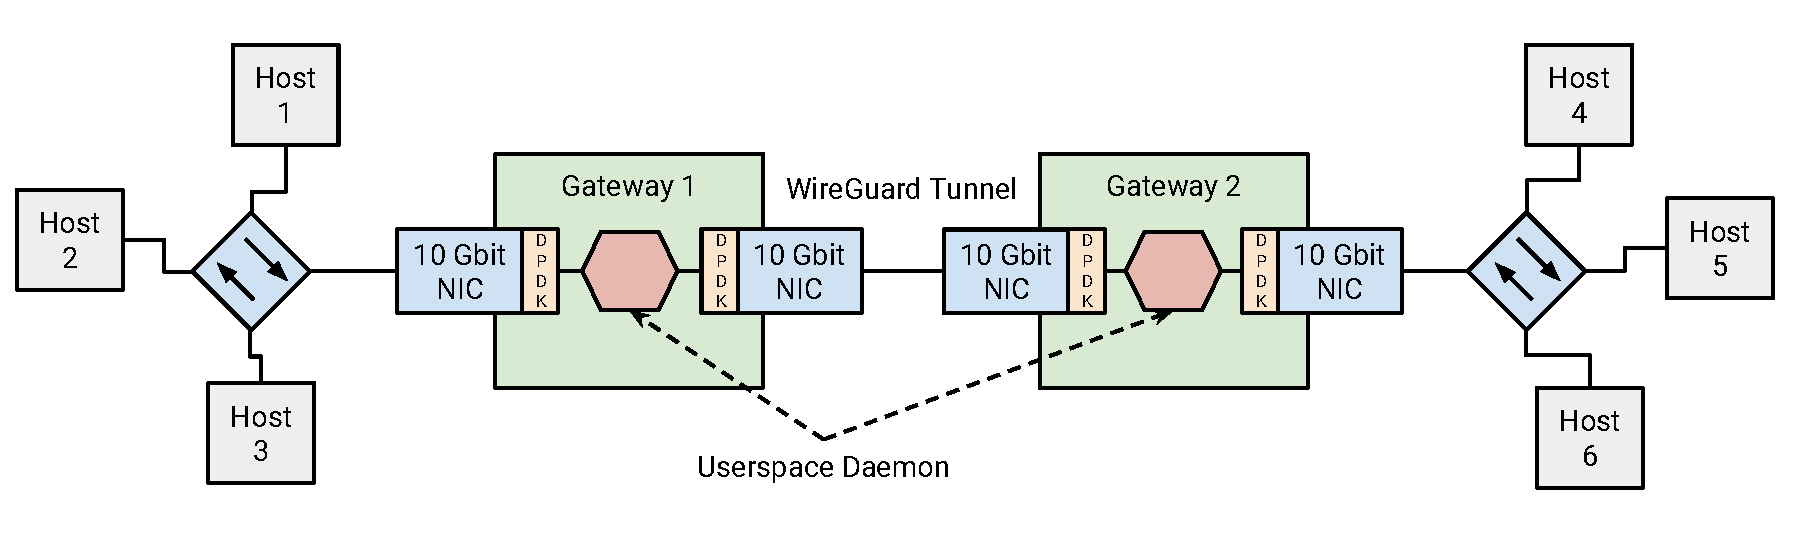
\includegraphics[width=1\linewidth]{figures/PoC-Overview}
		\caption{Overview of Site-to-Site VPN Setup}
		\label{fig:poc-overview}
	\end{figure}
	
	\subsubsection{Setup B - Many Client Entry Point}
	
	%TODO: sort by client or sort by benchmark?
	\subsection{IPsec}
	\subsection{OpenVPN}
	\subsection{WireGuard}
		\subsubsection{GSoC Performance Improvements}
	\subsection{MoonWire}
	\subsection{UDP Socket}

\chapter{Conclusion}
\label{chap:conclusion}
\section{Future Work}
	Implement better queuing: CODel

\appendix
\chapter{Supplementals}

\listoffigures
\listoftables

\chapter{Appendix}

foo


\printacronyms[heading=chapter,name=List of Acronyms]
\clearpage
\pagestyle{thesischapter}

\cleardoublepage
\printbibliography[heading=bibintoc]

%\cleardoublepage
\clearpage
\pagestyle{empty}
%\mbox{}
%\clearpage

\end{document}


